\documentclass[10pt]{extarticle}
\usepackage[a4paper,top=12mm,bottom=14mm,left=17mm,right=17mm]{geometry}
\usepackage[T1]{fontenc}
\usepackage{lmodern,microtype,graphicx,booktabs,tabularx,longtable,array,enumitem,amsmath,xcolor,titlesec,caption,fancyhdr,cite,hyperref}
\definecolor{ink}{HTML}{202124}
\definecolor{link}{HTML}{1F5A99}
\hypersetup{colorlinks=true,linkcolor=link,citecolor=link,urlcolor=link,pdfauthor={Alexander Suvorov},pdftitle={One Shot Is All You Need. Or Is It?}}
\urlstyle{same}
\graphicspath{{imgs/}}
\setlength{\parindent}{0pt}
\setlength{\parskip}{2.5pt}
\setlength{\tabcolsep}{3.5pt}
\renewcommand{\arraystretch}{1.10}
\setlist[itemize]{leftmargin=5mm,itemsep=1pt,topsep=2pt}
\titleformat{\section}{\large\bfseries\color{ink}}{\thesection}{0.45em}{}
\titleformat{\subsection}{\normalsize\bfseries\color{ink}}{\thesubsection}{0.4em}{}
\titlespacing*{\section}{0pt}{6pt}{2pt}
\titlespacing*{\subsection}{0pt}{4pt}{1pt}
\captionsetup{font=footnotesize,labelfont=bf,textfont=normalfont,skip=2pt}
\pagestyle{fancy}
\fancyhf{}
\fancyhead[L]{\scriptsize Alexander Suvorov}
\fancyhead[R]{\scriptsize One-shot SmolVLA adaptation}
\fancyfoot[C]{\scriptsize \thepage}
\renewcommand{\headrulewidth}{0.2pt}
\setlength{\headheight}{11pt}
\newcommand{\linkbutton}[2]{\href{#2}{\fbox{\strut\footnotesize\sffamily\bfseries #1}}}
\newcommand{\score}[3]{#1\% (#2/#3)}
\newcommand{\code}[1]{\texttt{\detokenize{#1}}}
\newcommand{\sha}[1]{\nolinkurl{#1}}
\newcommand{\artifact}[1]{\texttt{\footnotesize\detokenize{#1}}}
\newcommand{\figcap}[2]{\refstepcounter{figure}\label{#2}{\footnotesize\textbf{Figure \thefigure.} #1\par}}
\newcommand{\tabcap}[2]{\refstepcounter{table}\label{#2}{\footnotesize\textbf{Table \thetable.} #1\par}}
\newenvironment{finding}{\begin{center}\begin{minipage}{0.94\textwidth}\small\hrule\vspace{3pt}}{\vspace{3pt}\hrule\end{minipage}\end{center}}
\newcommand{\failurestrip}[3]{\begin{center}\includegraphics[width=0.84\textwidth]{#1}\\[-2pt]{\footnotesize\textbf{#2.} #3}\end{center}}

\begin{document}
\thispagestyle{empty}
\begin{center}
{\fontsize{20}{23}\selectfont\bfseries One Shot Is All You Need. Or Is It?}\\[2pt]
{\large Few-Shot SmolVLA Adaptation on LIBERO}\\[6pt]
{\normalsize\textbf{Alexander Suvorov}}\\[-1pt]
{\small HSE University \quad $\cdot$ \quad August 2026\textsuperscript{1}}\\[6pt]
\linkbutton{GitHub}{https://github.com/alexsuw/smolvla-libero-fewshot}\hspace{4pt}
\linkbutton{Hugging Face Models}{https://huggingface.co/collections/alexsuw/smolvla-libero-few-shot-6a8b009357482d2b4b9d3c2f}\hspace{4pt}
\linkbutton{LIBERO Dataset}{https://huggingface.co/datasets/nvidia/LIBERO_LeRobot_v3}
\end{center}
\footnotetext[1]{This work was prepared for the T-Lab 2026 VLA adaptation assignment.}

\section{Question and setup}
\begin{finding}
\textbf{How many demonstrations does SmolVLA need for a new task---and what does it forget while adapting?}
\end{finding}
I study SmolVLA, a compact vision-language-action policy \cite{smolvla2025},
on the LIBERO lifelong manipulation benchmark \cite{libero2023}. The setup is
intentionally simple:
\begin{itemize}
\item \textbf{Seen data:} all available \texttt{libero\_90}: 3,921 episodes, 569,249 frames, and 73 merged instructions.
\item \textbf{New tasks:} open the middle drawer, put the bowl on the stove, and put the wine bottle on top of the cabinet.
\item \textbf{Updated weights:} Action Expert and state/action projections; the vision encoder and VLM backbone stay frozen.
\item \textbf{Target metric:} binary simulator success over fixed rollouts.
\item \textbf{Retention metric:} the same metric on three frozen \texttt{libero\_90} probes.
\end{itemize}
I use the video-backed LeRobot conversion
\texttt{nvidia/LIBERO\_LeRobot\_v3} \cite{liberolerobotv3,lerobot}. Exact
revisions, episodes, seeds, statistics, and optimizer settings are in
Appendix~\ref{app:protocol}.

\section{First, build a working seen policy}
Starting from \texttt{lerobot/smolvla\_base}, I train the allowed 99.9M
parameters for 100k steps. The checkpoint is chosen only on frozen seen
probes, before looking at target success.
\begin{center}
\footnotesize
\begin{tabular}{@{}lccc@{}}
\toprule
Checkpoint & 60k & 80k & \textbf{100k}\\
\midrule
Seen probes & \score{70.0}{21}{30} & \score{76.7}{23}{30} & \textbf{\score{80.0}{24}{30}}\\
\bottomrule
\end{tabular}\\[-1pt]
\tabcap{Seen-only checkpoint selection.}{tab:seen-selection}
\end{center}
The 100k checkpoint has final loss 0.23494 and weights SHA-256 prefix
\texttt{2cd510a594a8}. The training trace is in Appendix~\ref{app:training}.

\section{Then, test zero-shot transfer}
The frozen policy almost does not solve the held-out tasks:
\textbf{\score{1.7}{1}{60}}. A paired language control uses the same initial
states with correct and wrong instructions. Correct language gives
\score{1.7}{1}{60}; wrong language gives \score{0.0}{0}{60}. Success is too
sparse for a strong claim, but action sequences change: mean paired \(L_2\)
distances are 0.582, 0.998, and 0.966 for Drawer, Bowl, and Wine.
Appendix~\ref{app:controls} gives the full control.
\begin{finding}
The seen policy works on its training suite, but it does not transfer to the
new tasks without adaptation. The next question is how quickly one new skill
can be acquired.
\end{finding}

\newpage
\section{One demonstration changes the problem}
The assignment first asks for \(N\in\{0,5,10,25\}\). Since \(N=5\) was near
the ceiling, I used the allowed extension and added \(N=1\) and \(N=2\).
Each cell uses the first \(N\) demos, train seeds 42 and 123, and 20 fixed
rollouts per seed. No demo is selected by success.
\begin{center}
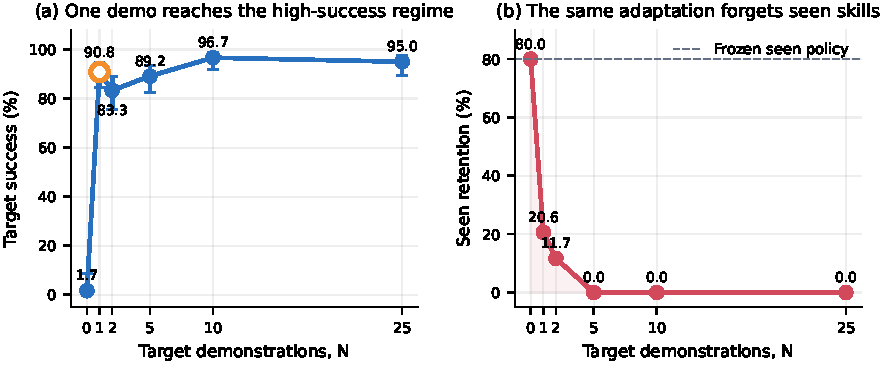
\includegraphics[width=0.98\textwidth]{discovery_summary.pdf}\\[-2pt]
\figcap{The naive target cost curve and corrected seen retention. Target error
bars are 95\% Wilson intervals.}{fig:discovery}
\end{center}
The main effect appears after one demonstration:
\textbf{\score{90.8}{109}{120}} target success, versus
\score{1.7}{1}{60} at zero shot. Ten demos give the best observed result,
\score{96.7}{116}{120}, but one shot is already in the high-success regime.
\(N=2\) is lower than \(N=1\), so the curve is not monotonic with two seeds.
\begin{center}
\footnotesize
\begin{tabular}{@{}rcc@{}}
\toprule
\(N\) & Target success & Seen retention\\
\midrule
0 & \score{1.7}{1}{60} & \score{80.0}{24}{30}\\
1 & \textbf{\score{90.8}{109}{120}} & \score{20.6}{37}{180}\\
2 & \score{83.3}{100}{120} & \score{11.7}{21}{180}\\
5 & \score{89.2}{107}{120} & \score{0.0}{0}{180}\\
10 & \score{96.7}{116}{120} & \score{0.0}{0}{180}\\
25 & \score{95.0}{114}{120} & \score{0.0}{0}{180}\\
\bottomrule
\end{tabular}\\[-1pt]
\tabcap{Naive adaptation. Exact cells are in Appendix~\ref{app:complete-results}.}{tab:naive-main}
\end{center}

\section{But what happened to the old skills?}
Figure~\ref{fig:discovery}b gives the second result. The frozen policy starts
at 80.0\% on seen probes. After one target demo, retention falls to 20.6\%;
at \(N\geq5\), it is 0.0\%. High target success and low retention happen
together.
The first retention run incorrectly used target-overlay statistics and gave
\score{0.0}{0}{900}. A 2-by-2 control showed that these statistics also break
the frozen seen policy. I therefore reran retention with original
\texttt{libero\_90} statistics. Appendix~\ref{app:normalization} keeps the
control and the rejected result.
\begin{finding}
\textbf{One demo is enough to learn the new task, but naive adaptation largely
overwrites the old policy.} Task 2 is now a stability question.
\end{finding}

\newpage
\section{Task 2: what can preserve the seen policy?}
\subsection{Parameter-efficient updates do not help}
Target-LoRA places rank-64 adapters in the Action Expert and keeps projections
trainable \cite{lora2022}. Replay-LoRA adds a 25\% stream sampled only from
\texttt{libero\_90}; it uses no other target demos and replay is not selected
by the probes.
\begin{center}
\footnotesize
\begin{tabular}{@{}lccc@{}}
\toprule
Method & Target success & Seen retention & Trainable\\
\midrule
Naive & \textbf{\score{90.8}{109}{120}} & \textbf{\score{20.6}{37}{180}} & 99.9M\\
Target-LoRA & \score{82.5}{99}{120} & \score{10.6}{19}{180} & 4.22M\\
Replay-LoRA & \score{55.8}{67}{120} & \score{1.1}{2}{180} & 4.22M\\
\bottomrule
\end{tabular}\\[-1pt]
\tabcap{The first preservation ideas. Parameter efficiency is not preservation.}{tab:lora-main}
\end{center}
Target-LoRA reduces trainable parameters 23.7 times, but both metrics get
worse. Replay-LoRA also mixes actions under incompatible target-only
normalization; Drawer loss explodes above \(10^{10}\). Details are in
Appendix~\ref{app:replay}.

\subsection{Does direct weight anchoring help?}
LoRA suggests a different hypothesis: forgetting may depend more on
\emph{where} the Action Expert moves than on how many parameters move.
Frozen-Stats FT uses canonical \texttt{libero\_90} statistics with no extra
penalty. Anchored FT adds L2-SP \cite{l2sp2018}:
\[
\mathcal{L}=\mathcal{L}_{\mathrm{target}}+
\lambda\sum_{\theta_i\in\Theta_{\mathrm{train}}}
\left\lVert\theta_i-\theta_{i,\mathrm{seen}}\right\rVert_2^2,
\qquad \lambda=0.01.
\]
Here \(\theta_{i,\mathrm{seen}}\) is the frozen 100k initialization. The
penalty keeps trainable weights near the seen policy. The single deterministic
\(\lambda\) was locked before evaluation and was not swept.
\begin{center}
\footnotesize
\begin{tabular}{@{}lcccccc@{}}
\toprule
Method & Target & Retain & \(\Delta\)target & \(\Delta\)retain & Wall & VRAM\\
\midrule
Naive & 90.8\% & 20.6\% & -- & -- & 162.8s & 7,540 MiB\\
Frozen-Stats & 90.8\% & 21.7\% & +0.0 pp & +1.1 pp & 311.3s & 7,540 MiB\\
\textbf{L2-SP} & \textbf{87.5\%} & \textbf{31.7\%} & \textbf{-3.3 pp} &
\textbf{+11.1 pp} & 297.3s & 8,036 MiB\\
\bottomrule
\end{tabular}\\[-1pt]
\tabcap{Matched \(N=1\) comparison. Naive was reused, not rerun.}{tab:l2sp-main}
\end{center}
\begin{center}
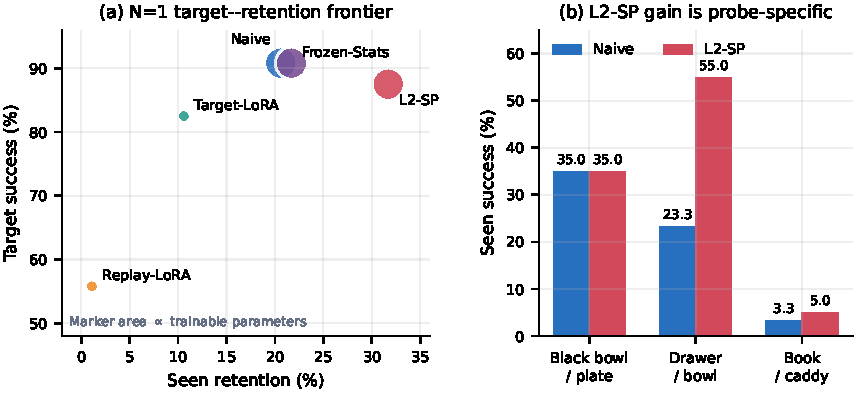
\includegraphics[width=0.98\textwidth]{method_story.pdf}\\[-2pt]
\figcap{Updated \(N=1\) frontier and frozen-probe breakdown. Marker area in
panel (a) is proportional to trainable parameters.}{fig:method-story}
\end{center}
Frozen statistics alone change little. L2-SP gains 11.1 retention points for
3.3 target points. It is a useful Pareto trade-off, not strict dominance.
Also, 19 of its 20 extra retained successes come from
\texttt{drawer\_bowl}. This supports anchoring, but not broad LIBERO-90
preservation. Appendix~\ref{app:n1-cells} reports every task and seed.

\newpage
\section{Failures, predictions, and conclusion}
These are real failed zero-shot rollouts at seed 1000. Frames are at 0, 5, 10,
and 15 seconds; no successful video was selected.
\failurestrip{failure_drawer.jpg}{Drawer}{The arm does not approach the middle drawer handle.}
\failurestrip{failure_bowl.jpg}{Bowl}{The arm reaches the dish area but does not complete grasp and placement.}
\failurestrip{failure_wine.jpg}{Wine}{The first reach goes toward a distractor; the bottle is not picked up.}

\textbf{Separating tests.}
For Drawer, compare the original image with a handle crop or point marker.
For Bowl, compare a normal start with the bowl already grasped. For Wine,
cross an object-colour swap with a grasped start. These tests separate
grounding, grasping, identity, and placement failures; details are in
Appendix~\ref{app:failure-tests}.

\textbf{Predictions versus results.}
I correctly expected the largest gain before five demos and later saturation.
I incorrectly expected Replay-LoRA \(>\) Target-LoRA \(>\) naive. The actual
order was the reverse. A small update can still interfere with old skills,
and replay is unsafe when action scales are inconsistent.

\textbf{Idea graveyard.}
I rejected target-task hyperparameter sweeps, target-overlay statistics for
seen deployment, and full-VLM fine-tuning. These would tune on test tasks,
confound retention, or add compute without testing the key question.
\begin{finding}
\textbf{Most surprising result.}
One demo reaches 90.8\% target success, but naive adaptation leaves 20.6\%
retention. Parameter efficiency does not solve this. Weight anchoring recovers
part of the old behaviour: 31.7\% retention at 87.5\% target success.
\end{finding}
The evidence is limited to three target tasks, two train seeds, and three
retention probes. The next experiment should use a preregistered broader
retention panel for the existing Naive and L2-SP checkpoints, then add train
seeds. Future \(\lambda\) comparisons should use separate calibration tasks.

All 600 new rollouts were independently recounted. Hashes, demo IDs, seeds,
and the canonical statistics digest match; \texttt{integrity\_ok=true}.
The full suite reports 304 passed, 8 skipped, and 0 failed. Exact protocols,
tables, curves, hashes, and artifact paths follow in this same PDF.

\clearpage
\appendix
\setcounter{section}{0}
\setcounter{figure}{0}
\setcounter{table}{0}
\renewcommand{\thefigure}{A\arabic{figure}}
\renewcommand{\thetable}{A\arabic{table}}
\renewcommand{\theHfigure}{appendix.\arabic{figure}}
\renewcommand{\theHtable}{appendix.\arabic{table}}
\renewcommand{\thepage}{A-\arabic{page}}
\setcounter{page}{1}
\fancyhead[R]{\scriptsize Technical Appendix}
\begin{center}
{\fontsize{18}{21}\selectfont\bfseries Technical Appendix}\\[2pt]
{\large One Shot Is All You Need. Or Is It?}\\[4pt]
{\small Alexander Suvorov, HSE University}
\end{center}
This appendix is part of the same source file and PDF as the four-page main
report. It records the complete protocol, percentages and raw counts,
training curves, compute, controls, hashes, and artifact map.

\section{Frozen protocol and provenance}
\label{app:protocol}

\subsection{Immutable sources}
\begin{center}
\footnotesize
\begin{tabularx}{\textwidth}{@{}lX@{}}
\toprule
Item & Frozen value\\
\midrule
Base model & \code{lerobot/smolvla_base}, revision
\sha{c83c3163b8ca9b7e67c509fffd9121e66cb96205}\\
Dataset & \code{nvidia/LIBERO_LeRobot_v3}, revision
\sha{e5907374380b8f96511957e6ba5582be52a1e179}\\
Seen data & Full available \code{libero_90}: 3,921 episodes, 569,249 frames,
73 instruction rows\\
Seen checkpoint & \code{step_100000}; weights SHA-256
\sha{2cd510a594a87580f7368b782ca9b37332c0e5002d807093c759e95fbfb57c88}\\
Seen statistics & \code{libero_90}; digest
\sha{b159b6fed3e52edf25bd39b377dd64940221b7a030362daf7f726b1c2ecb30cf}\\
First \(N=1\) episodes & Drawer 20; Bowl 13; Wine 6\\
Train seeds & 42 and 123\\
Target evaluation & Seeds 1000--1019; 20 rollouts per checkpoint\\
Retention & \code{black_bowl_plate}, \code{drawer_bowl}, \code{book_caddy};
seeds 1000--1009; canonical \code{libero_90} statistics\\
Environment & Hard reset, relative control, 300-step horizon; predict 50
actions and execute 10\\
\bottomrule
\end{tabularx}\\[-1pt]
\tabcap{Frozen data, checkpoint, and evaluation protocol.}{tab:provenance}
\end{center}

Target tasks are held out by exact instruction text: \emph{open the middle
drawer of the cabinet}, \emph{put the bowl on the stove}, and \emph{put the
wine bottle on top of the cabinet}. They are not selected by dataset row
number.

\subsection{Training settings}
The vision encoder and VLM backbone stay frozen. Naive, Frozen-Stats, and
L2-SP train the Action Expert plus state/action projections: exactly
99,880,992 parameters. Target-LoRA and Replay-LoRA use rank \(r=64\),
\(\alpha=64\), zero dropout, plus projections: 4,215,632 parameters.

\begin{center}
\footnotesize
\begin{tabular}{@{}lrrlll@{}}
\toprule
Stage & Learning rate & Maximum & Stop rule & Batch & Precision\\
\midrule
Seen expert & \(10^{-4}\) & 100,000 & fixed & 32 & bf16\\
Naive target & \(10^{-4}\) & 12,000 & min(100 epochs, cap) & 32 & bf16\\
Target-LoRA & \(10^{-3}\) & 12,000 & min(100 epochs, cap) & 32 & bf16\\
Replay-LoRA & \(10^{-3}\) & 12,000 & min(100 epochs, cap) & 32 & bf16\\
Frozen-Stats & \(10^{-4}\) & 12,000 & min(100 epochs, cap) & 32 & bf16\\
L2-SP & \(10^{-4}\) & 12,000 & same + \(\lambda=0.01\) & 32 & bf16\\
\bottomrule
\end{tabular}\\[-1pt]
\tabcap{Training recipes. No method uses success-based stopping or reruns.}{tab:training-recipe}
\end{center}

All runs use AdamW, weight decay \(10^{-2}\), betas \((0.9,0.95)\), gradient
clipping at 1.0, 1,000-step warm-up, and cosine decay. Replay draws 75\%
target and 25\% \code{libero_90}. Frozen-Stats and L2-SP use only the first
target demo and canonical seen statistics. L2-SP computes the raw-sum anchor
penalty in FP32 against the frozen seen initialization.

The gripper conversion is
\(a_{\mathrm{env}}=1-2a_{\mathrm{data}}\). Six stored demonstrations replay
with \score{100.0}{6}{6} success. The matched preflight found finite normalized
actions and gripper range \([-1.059968,0.943425]\).

\clearpage

\section{Complete evaluation results}
\label{app:complete-results}

\subsection{Naive target cost curve}
\begin{center}
\footnotesize
\begin{tabular}{@{}rccccccc@{}}
\toprule
\(N\) & Drawer 42 & Drawer 123 & Bowl 42 & Bowl 123 & Wine 42 & Wine 123 & Pooled\\
\midrule
0 & \multicolumn{2}{c}{\score{5.0}{1}{20}} &
\multicolumn{2}{c}{\score{0.0}{0}{20}} &
\multicolumn{2}{c}{\score{0.0}{0}{20}} & \score{1.7}{1}{60}\\
1 & \score{85.0}{17}{20} & \score{95.0}{19}{20} &
\score{100.0}{20}{20} & \score{100.0}{20}{20} &
\score{80.0}{16}{20} & \score{85.0}{17}{20} & \score{90.8}{109}{120}\\
2 & \score{50.0}{10}{20} & \score{100.0}{20}{20} &
\score{100.0}{20}{20} & \score{90.0}{18}{20} &
\score{80.0}{16}{20} & \score{80.0}{16}{20} & \score{83.3}{100}{120}\\
5 & \score{85.0}{17}{20} & \score{70.0}{14}{20} &
\score{100.0}{20}{20} & \score{100.0}{20}{20} &
\score{85.0}{17}{20} & \score{95.0}{19}{20} & \score{89.2}{107}{120}\\
10 & \score{95.0}{19}{20} & \score{100.0}{20}{20} &
\score{100.0}{20}{20} & \score{100.0}{20}{20} &
\score{95.0}{19}{20} & \score{90.0}{18}{20} & \score{96.7}{116}{120}\\
25 & \score{100.0}{20}{20} & \score{100.0}{20}{20} &
\score{100.0}{20}{20} & \score{100.0}{20}{20} &
\score{80.0}{16}{20} & \score{90.0}{18}{20} & \score{95.0}{114}{120}\\
\bottomrule
\end{tabular}\\[-1pt]
\tabcap{All naive target cells. Every success entry gives percentage and raw count.}{tab:naive-full}
\end{center}

\begin{center}
\footnotesize
\begin{tabular}{@{}rccc@{}}
\toprule
\(N\) & Target success & 95\% Wilson interval & Change from zero shot\\
\midrule
0 & \score{1.7}{1}{60} & [0.3, 8.9]\% & --\\
1 & \score{90.8}{109}{120} & [84.3, 94.8]\% & +89.2 pp\\
2 & \score{83.3}{100}{120} & [75.7, 88.9]\% & +81.7 pp\\
5 & \score{89.2}{107}{120} & [82.3, 93.6]\% & +87.5 pp\\
10 & \score{96.7}{116}{120} & [91.7, 98.7]\% & +95.0 pp\\
25 & \score{95.0}{114}{120} & [89.5, 97.7]\% & +93.3 pp\\
\bottomrule
\end{tabular}\\[-1pt]
\tabcap{Pooled target curve with uncertainty.}{tab:naive-ci}
\end{center}

\subsection{Corrected seen retention}
\begin{center}
\footnotesize
\begin{tabular}{@{}rccccc@{}}
\toprule
\(N\) & Drawer-trained & Bowl-trained & Wine-trained & Pooled & Change\\
\midrule
0 & \multicolumn{3}{c}{Frozen reference \score{80.0}{24}{30}} &
\score{80.0}{24}{30} & --\\
1 & \score{10.0}{6}{60} & \score{33.3}{20}{60} & \score{18.3}{11}{60} &
\score{20.6}{37}{180} & -59.4 pp\\
2 & \score{8.3}{5}{60} & \score{21.7}{13}{60} & \score{5.0}{3}{60} &
\score{11.7}{21}{180} & -68.3 pp\\
5 & \score{0.0}{0}{60} & \score{0.0}{0}{60} & \score{0.0}{0}{60} &
\score{0.0}{0}{180} & -80.0 pp\\
10 & \score{0.0}{0}{60} & \score{0.0}{0}{60} & \score{0.0}{0}{60} &
\score{0.0}{0}{180} & -80.0 pp\\
25 & \score{0.0}{0}{60} & \score{0.0}{0}{60} & \score{0.0}{0}{60} &
\score{0.0}{0}{180} & -80.0 pp\\
\bottomrule
\end{tabular}\\[-1pt]
\tabcap{Corrected retention with canonical \texttt{libero\_90} statistics.}{tab:retention-full}
\end{center}

Across the 30 adapted naive cells, target success and corrected retention have
Pearson \(r=0.026\). This is descriptive because cells share tasks.

\clearpage

\subsection{All matched \texorpdfstring{\(N=1\)}{N=1} cells}
\label{app:n1-cells}
Target uses 20 rollouts. Retention uses 30 rollouts: three probes and ten
fixed seeds. All success cells give percentage and raw count.

{\footnotesize
\begin{longtable}{@{}llrllll@{}}
\caption{Every matched \(N=1\) task, seed, result, wall time, and peak VRAM.}
\label{tab:all-n1}\\
\toprule
Method & Target task & Seed & Target & Retention & Train wall & Peak VRAM\\
\midrule
\endfirsthead
\toprule
Method & Target task & Seed & Target & Retention & Train wall & Peak VRAM\\
\midrule
\endhead
Naive & Drawer & 42 & \score{85.0}{17}{20} & \score{13.3}{4}{30} & 199.1s & 7,540 MiB\\
Naive & Drawer & 123 & \score{95.0}{19}{20} & \score{6.7}{2}{30} & 199.4s & 7,540 MiB\\
Naive & Bowl & 42 & \score{100.0}{20}{20} & \score{33.3}{10}{30} & 162.2s & 7,540 MiB\\
Naive & Bowl & 123 & \score{100.0}{20}{20} & \score{33.3}{10}{30} & 162.0s & 7,540 MiB\\
Naive & Wine & 42 & \score{80.0}{16}{20} & \score{20.0}{6}{30} & 127.2s & 7,540 MiB\\
Naive & Wine & 123 & \score{85.0}{17}{20} & \score{16.7}{5}{30} & 126.9s & 7,540 MiB\\
\midrule
Target-LoRA & Drawer & 42 & \score{75.0}{15}{20} & \score{0.0}{0}{30} & 314.7s & 6,944 MiB\\
Target-LoRA & Drawer & 123 & \score{40.0}{8}{20} & \score{3.3}{1}{30} & 315.0s & 6,938 MiB\\
Target-LoRA & Bowl & 42 & \score{100.0}{20}{20} & \score{30.0}{9}{30} & 229.7s & 6,944 MiB\\
Target-LoRA & Bowl & 123 & \score{100.0}{20}{20} & \score{23.3}{7}{30} & 229.3s & 6,944 MiB\\
Target-LoRA & Wine & 42 & \score{95.0}{19}{20} & \score{3.3}{1}{30} & 187.0s & 6,882 MiB\\
Target-LoRA & Wine & 123 & \score{85.0}{17}{20} & \score{3.3}{1}{30} & 188.2s & 6,944 MiB\\
\midrule
Replay-LoRA & Drawer & 42 & \score{15.0}{3}{20} & \score{0.0}{0}{30} & 435.9s & 6,944 MiB\\
Replay-LoRA & Drawer & 123 & \score{15.0}{3}{20} & \score{0.0}{0}{30} & 436.0s & 6,944 MiB\\
Replay-LoRA & Bowl & 42 & \score{100.0}{20}{20} & \score{3.3}{1}{30} & 332.3s & 6,944 MiB\\
Replay-LoRA & Bowl & 123 & \score{100.0}{20}{20} & \score{3.3}{1}{30} & 332.3s & 6,944 MiB\\
Replay-LoRA & Wine & 42 & \score{40.0}{8}{20} & \score{0.0}{0}{30} & 159.7s & 6,944 MiB\\
Replay-LoRA & Wine & 123 & \score{65.0}{13}{20} & \score{0.0}{0}{30} & 159.9s & 6,944 MiB\\
\midrule
Frozen-Stats & Drawer & 42 & \score{100.0}{20}{20} & \score{13.3}{4}{30} & 378.3s & 7,540 MiB\\
Frozen-Stats & Drawer & 123 & \score{100.0}{20}{20} & \score{13.3}{4}{30} & 376.9s & 7,540 MiB\\
Frozen-Stats & Bowl & 42 & \score{100.0}{20}{20} & \score{13.3}{4}{30} & 326.1s & 7,540 MiB\\
Frozen-Stats & Bowl & 123 & \score{100.0}{20}{20} & \score{16.7}{5}{30} & 325.5s & 7,540 MiB\\
Frozen-Stats & Wine & 42 & \score{75.0}{15}{20} & \score{40.0}{12}{30} & 230.4s & 7,540 MiB\\
Frozen-Stats & Wine & 123 & \score{70.0}{14}{20} & \score{33.3}{10}{30} & 230.4s & 7,540 MiB\\
\midrule
L2-SP & Drawer & 42 & \score{100.0}{20}{20} & \score{23.3}{7}{30} & 392.3s & 8,036 MiB\\
L2-SP & Drawer & 123 & \score{100.0}{20}{20} & \score{23.3}{7}{30} & 392.3s & 8,036 MiB\\
L2-SP & Bowl & 42 & \score{95.0}{19}{20} & \score{23.3}{7}{30} & 314.8s & 8,036 MiB\\
L2-SP & Bowl & 123 & \score{85.0}{17}{20} & \score{33.3}{10}{30} & 314.7s & 8,036 MiB\\
L2-SP & Wine & 42 & \score{70.0}{14}{20} & \score{40.0}{12}{30} & 185.2s & 8,036 MiB\\
L2-SP & Wine & 123 & \score{75.0}{15}{20} & \score{46.7}{14}{30} & 184.5s & 8,036 MiB\\
\bottomrule
\end{longtable}
}

\subsection{Aggregate intervals and probe totals}
\begin{center}
\footnotesize
\begin{tabular}{@{}lcccc@{}}
\toprule
Method & Target & 95\% CI & Retention & 95\% CI\\
\midrule
Naive & \score{90.8}{109}{120} & [84.3,94.8]\% & \score{20.6}{37}{180} & [15.3,27.0]\%\\
Target-LoRA & \score{82.5}{99}{120} & [74.7,88.3]\% & \score{10.6}{19}{180} & [6.9,15.9]\%\\
Replay-LoRA & \score{55.8}{67}{120} & [46.9,64.4]\% & \score{1.1}{2}{180} & [0.3,4.0]\%\\
Frozen-Stats & \score{90.8}{109}{120} & [84.3,94.8]\% & \score{21.7}{39}{180} & [16.3,28.2]\%\\
L2-SP & \score{87.5}{105}{120} & [80.4,92.3]\% & \score{31.7}{57}{180} & [25.3,38.8]\%\\
\bottomrule
\end{tabular}\\[-1pt]
\tabcap{Matched \(N=1\) aggregate results and Wilson intervals.}{tab:n1-ci}
\end{center}

\begin{center}
\footnotesize
\begin{tabular}{@{}lccc@{}}
\toprule
Method & Black bowl / plate & Drawer / bowl & Book / caddy\\
\midrule
Naive & \score{35.0}{21}{60} & \score{23.3}{14}{60} & \score{3.3}{2}{60}\\
Target-LoRA & \score{20.0}{12}{60} & \score{11.7}{7}{60} & \score{0.0}{0}{60}\\
Replay-LoRA & \score{3.3}{2}{60} & \score{0.0}{0}{60} & \score{0.0}{0}{60}\\
Frozen-Stats & \score{25.0}{15}{60} & \score{36.7}{22}{60} & \score{3.3}{2}{60}\\
L2-SP & \score{35.0}{21}{60} & \score{55.0}{33}{60} & \score{5.0}{3}{60}\\
\bottomrule
\end{tabular}\\[-1pt]
\tabcap{Retention totals by frozen probe.}{tab:probe-totals}
\end{center}

\clearpage

\section{Training diagnostics}
\label{app:training}

\subsection{Seen expert}
The 100k run takes 38,870 seconds (10 h 47 min 50 s), processes 3.2M samples,
reserves 7,536 MiB at the final logged step, and ends at loss 0.23494.
\begin{center}
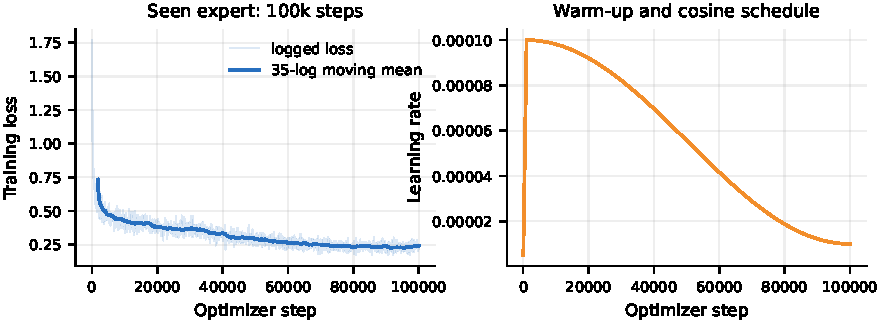
\includegraphics[width=\textwidth]{seen_training.pdf}\\[-2pt]
\figcap{Seen-expert loss, moving mean, warm-up, and cosine schedule.}{fig:seen-train}
\end{center}

\subsection{Naive target training}
The stop rule is 100 dataset epochs capped at 12k steps. At \(N=1\), final
steps are 500 for Drawer, 400 for Bowl, and 300 for Wine.
\begin{center}
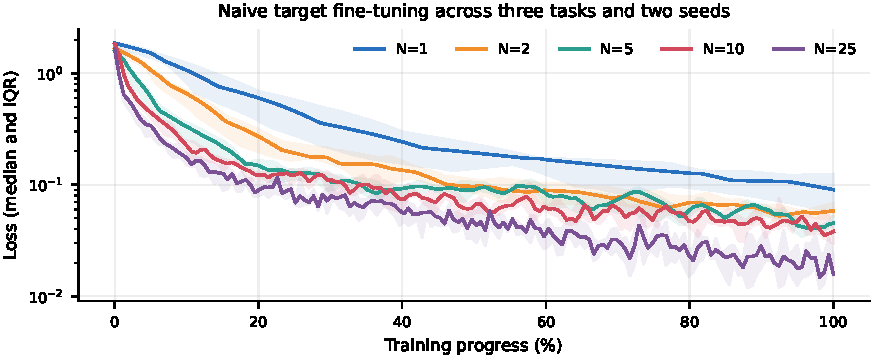
\includegraphics[width=\textwidth]{baseline_training.pdf}\\[-2pt]
\figcap{Naive target loss for all budgets. Curves show the median and
interquartile range across three tasks and two seeds.}{fig:baseline-train}
\end{center}

\subsection{LoRA and replay diagnostics}
\label{app:replay}
\begin{center}
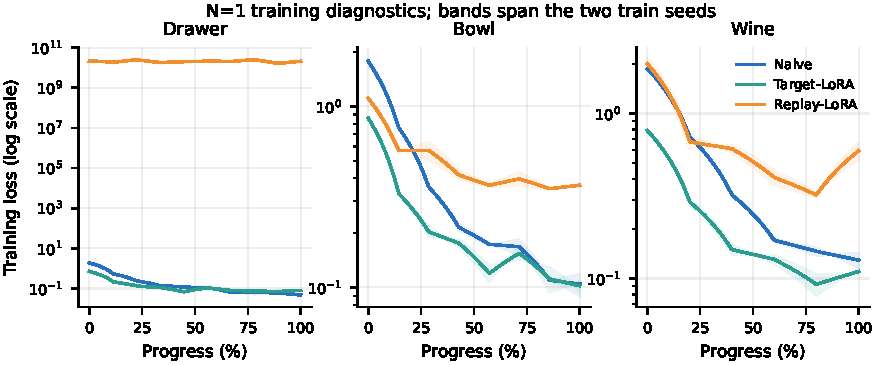
\includegraphics[width=\textwidth]{lora_diagnostics.pdf}\\[-2pt]
\figcap{\(N=1\) training by task for Naive, Target-LoRA, and Replay-LoRA.}{fig:lora-train}
\end{center}
Replay-LoRA Drawer is numerically pathological. The first target demo has
gripper standard deviation \(10^{-6}\), while seen replay has both states.
Target-only normalization creates extreme replay targets. Final Drawer losses
are \(1.44\times10^{10}\) and \(2.72\times10^{10}\). Bowl and Wine do not
show the same explosion, so this does not explain every lost seen success.

\subsection{Frozen-Stats and L2-SP diagnostics}
\begin{center}
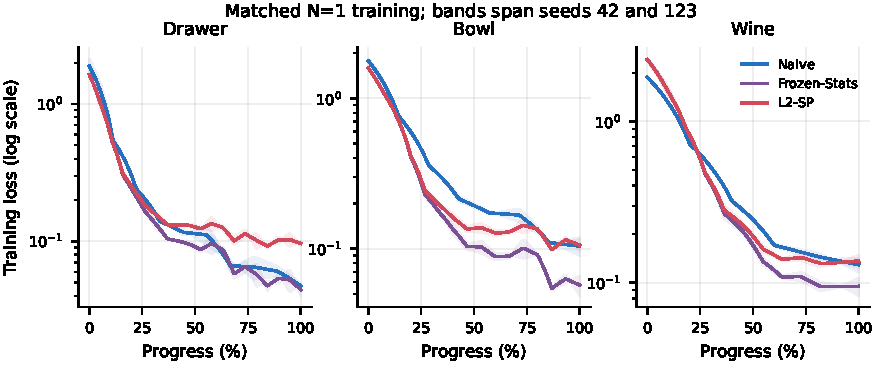
\includegraphics[width=\textwidth]{matched_diagnostics.pdf}\\[-2pt]
\figcap{Matched \(N=1\) loss curves. L2-SP includes the fixed anchor penalty;
bands span seeds 42 and 123.}{fig:matched-train}
\end{center}

\begin{center}
\footnotesize
\begin{tabular}{@{}llrrr@{}}
\toprule
Method & Cell & Final step & Samples & Final logged loss\\
\midrule
Frozen-Stats & Drawer 42 / 123 & 500 & 16,000 & 0.03646 / 0.05225\\
Frozen-Stats & Bowl 42 / 123 & 400 & 12,800 & 0.04071 / 0.07398\\
Frozen-Stats & Wine 42 / 123 & 300 & 9,600 & 0.07232 / 0.11800\\
L2-SP & Drawer 42 / 123 & 500 & 16,000 & 0.09008 / 0.10256\\
L2-SP & Bowl 42 / 123 & 400 & 12,800 & 0.08710 / 0.12436\\
L2-SP & Wine 42 / 123 & 300 & 9,600 & 0.11272 / 0.16037\\
\bottomrule
\end{tabular}\\[-1pt]
\tabcap{Exact final records for the matched training cells.}{tab:matched-loss}
\end{center}

\subsection{Compute, concurrency, and end-to-end time}
\begin{center}
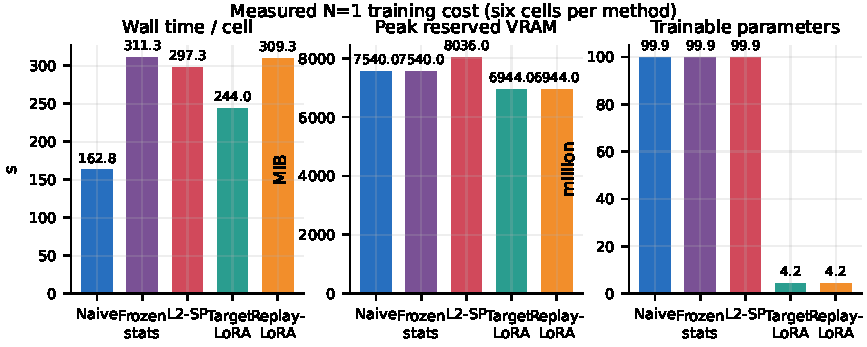
\includegraphics[width=\textwidth]{compute_cost.pdf}\\[-2pt]
\figcap{Mean wall time per cell, peak reserved VRAM, and trainable parameters.}{fig:compute}
\end{center}
For the matched grid, two jobs reach 194.0 aggregate samples/s and four reach
202.7 samples/s (+4.4\%). Four-way concurrency was safe and reserved about
33--35 GiB of the 97.9 GiB GPU.

The matched 12-cell grid took 47 min 39 s: training 15 min 57 s, target
evaluation 8 min 58 s, and retention 22 min 44 s. Including action audit,
smokes, and concurrency checks, the run took about 58 minutes. There were no
failed stages.

\clearpage

\section{Controls and integrity}

\subsection{Language control}
\label{app:controls}
\begin{center}
\footnotesize
\begin{tabular}{@{}lccc@{}}
\toprule
Task & Correct instruction & Wrong instruction & Mean action \(L_2\)\\
\midrule
Drawer & \score{5.0}{1}{20} & \score{0.0}{0}{20} & 0.5820\\
Bowl & \score{0.0}{0}{20} & \score{0.0}{0}{20} & 0.9982\\
Wine & \score{0.0}{0}{20} & \score{0.0}{0}{20} & 0.9661\\
\bottomrule
\end{tabular}\\[-1pt]
\tabcap{Paired control on identical initial-state fingerprints.}{tab:language}
\end{center}
Mean cosine gaps are 0.3273, 0.7731, and 0.6626. Changed trajectories show
language sensitivity, but low success does not prove strong zero-shot
instruction understanding.

\subsection{Normalization 2-by-2 control}
\label{app:normalization}
\begin{center}
\footnotesize
\begin{tabular}{@{}llcc@{}}
\toprule
Weights & Statistics & Success & Interpretation\\
\midrule
Frozen seen & \code{libero_90} & \score{80.0}{12}{15} & expected competence\\
Frozen seen & target overlay & \score{0.0}{0}{60} & statistics break deployment\\
Adapted target & target overlay & \score{0.0}{0}{60} & confounded old result\\
Adapted target & \code{libero_90} & \score{10.0}{6}{60} & corrected weight test\\
\bottomrule
\end{tabular}\\[-1pt]
\tabcap{Control separating weight change from statistics change.}{tab:norm-control}
\end{center}
The earlier \score{0.0}{0}{900} result is kept only as a deployment warning,
not as evidence of catastrophic forgetting.

\subsection{Matched-run integrity}
All 12 matched checkpoints have distinct final weight hashes. The 240 target
and 360 retention records were independently recounted from raw JSONL:
Frozen-Stats gives \score{90.8}{109}{120} and \score{21.7}{39}{180}; L2-SP
gives \score{87.5}{105}{120} and \score{31.7}{57}{180}. Every record matches
the registered task, demo episode, train seed, evaluation seed, checkpoint
hash, and canonical statistics digest. The driver reports
\texttt{integrity\_ok=true} and zero failed stages.

Implementation commit:
\sha{f77c469c5f90a2b7bba37988b39848b0b7101abe}.\par
Results commit:
\sha{66f04e9beaaa74e074e6aecb49ffb47bfd7bc3c6}.\par
The full suite reports 304 passed, 8 skipped, and 0 failed.

\section{Failure hypotheses and separating tests}
\label{app:failure-tests}
\textbf{Drawer: spatial grounding or low-level control?}
Compare the original image, a handle crop, and a point-marked image while
keeping state and instruction fixed. Measure end-effector distance to the
middle handle before contact. Improvement only with visual guidance supports
a grounding failure.

\textbf{Bowl: grasping or relational planning?}
Use two matched starts: the normal scene and the same scene with the bowl
already in the gripper. Success only from the second start isolates grasping;
failure in both supports a placement or long-horizon problem.

\textbf{Wine: object identity or placement horizon?}
Cross two interventions: swap bottle and distractor colours, and start with
the bottle already grasped. A reach that follows colour supports an identity
error; failure from the grasped start points to cabinet-top placement.

\clearpage
\section{Artifact map and next experiment}
\begin{center}
\footnotesize
\begin{tabularx}{\textwidth}{@{}lX@{}}
\toprule
Evidence & Location\\
\midrule
Unified source & \artifact{report/latex/paper.tex}\\
Compiled paper and appendix & \artifact{report/latex/build/paper.pdf}\\
Frozen predictions & \artifact{predictions.md}\\
Naive \(N=1,2\) & \artifact{/mnt/vla/validation/TODO28_n12/results.md}\\
Corrected naive retention &
\artifact{/mnt/vla/validation/TODO28_retention_libero90/retention.md}\\
LoRA result & \artifact{report/tables/task2_n1_results.md}\\
Frozen-Stats/L2-SP & \artifact{report/tables/frozen_stats_l2sp_n1_results.md}\\
Matched summary & \artifact{/mnt/vla/validation/TODO32/summary.json}\\
Matched checkpoints & \artifact{/mnt/vla/runs/target_matched_n1}\\
Matched target evaluation & \artifact{/mnt/vla/eval/target_matched_n1}\\
Matched retention & \artifact{/mnt/vla/eval/seen_retention_libero90_matched_n1}\\
\bottomrule
\end{tabularx}\\[-1pt]
\tabcap{Source and evidence locations. Runtime paths are on the experiment
host; portable summaries are committed.}{tab:artifacts}
\end{center}

The next locked experiment should evaluate existing Naive and L2-SP
checkpoints on a broader, preregistered seen-task panel. This tests whether the
gain extends beyond \texttt{drawer\_bowl}. If it does, add train seeds. Any
future \(\lambda\) values should be chosen on separate calibration tasks.
Useful mechanistic follow-ups are parameter drift by Action Expert component
and a matched function-space distillation penalty.

\section{References}
{\footnotesize
\bibliographystyle{unsrt}
\bibliography{references}
}


\end{document}
